\documentclass{article}
% To include code color syntaxing
\usepackage{minted}
% To include images
\usepackage{graphicx}
% To define margins
\usepackage[a4paper,left=2.5cm,right=2.5cm,top=2.5cm,bottom=2.5cm]{geometry}
% To comment multiple lines
\usepackage{comment}
% To use hyperlink
\usepackage{hyperref}
% Setting all hyperlinks color to black, then setting only url colors to blue
\hypersetup{
  colorlinks,
  allcolors=.,
  urlcolor=blue,
}

\begin{document}

\begin{titlepage}
	\begin{center}
		\huge{\bfseries II.2315 – Project : Advanced algorithm and programming} \\
		\rule{16cm}{0.4pt} \\
		\huge{\bfseries Australia - Canberra} \\
		\vspace{3mm}
		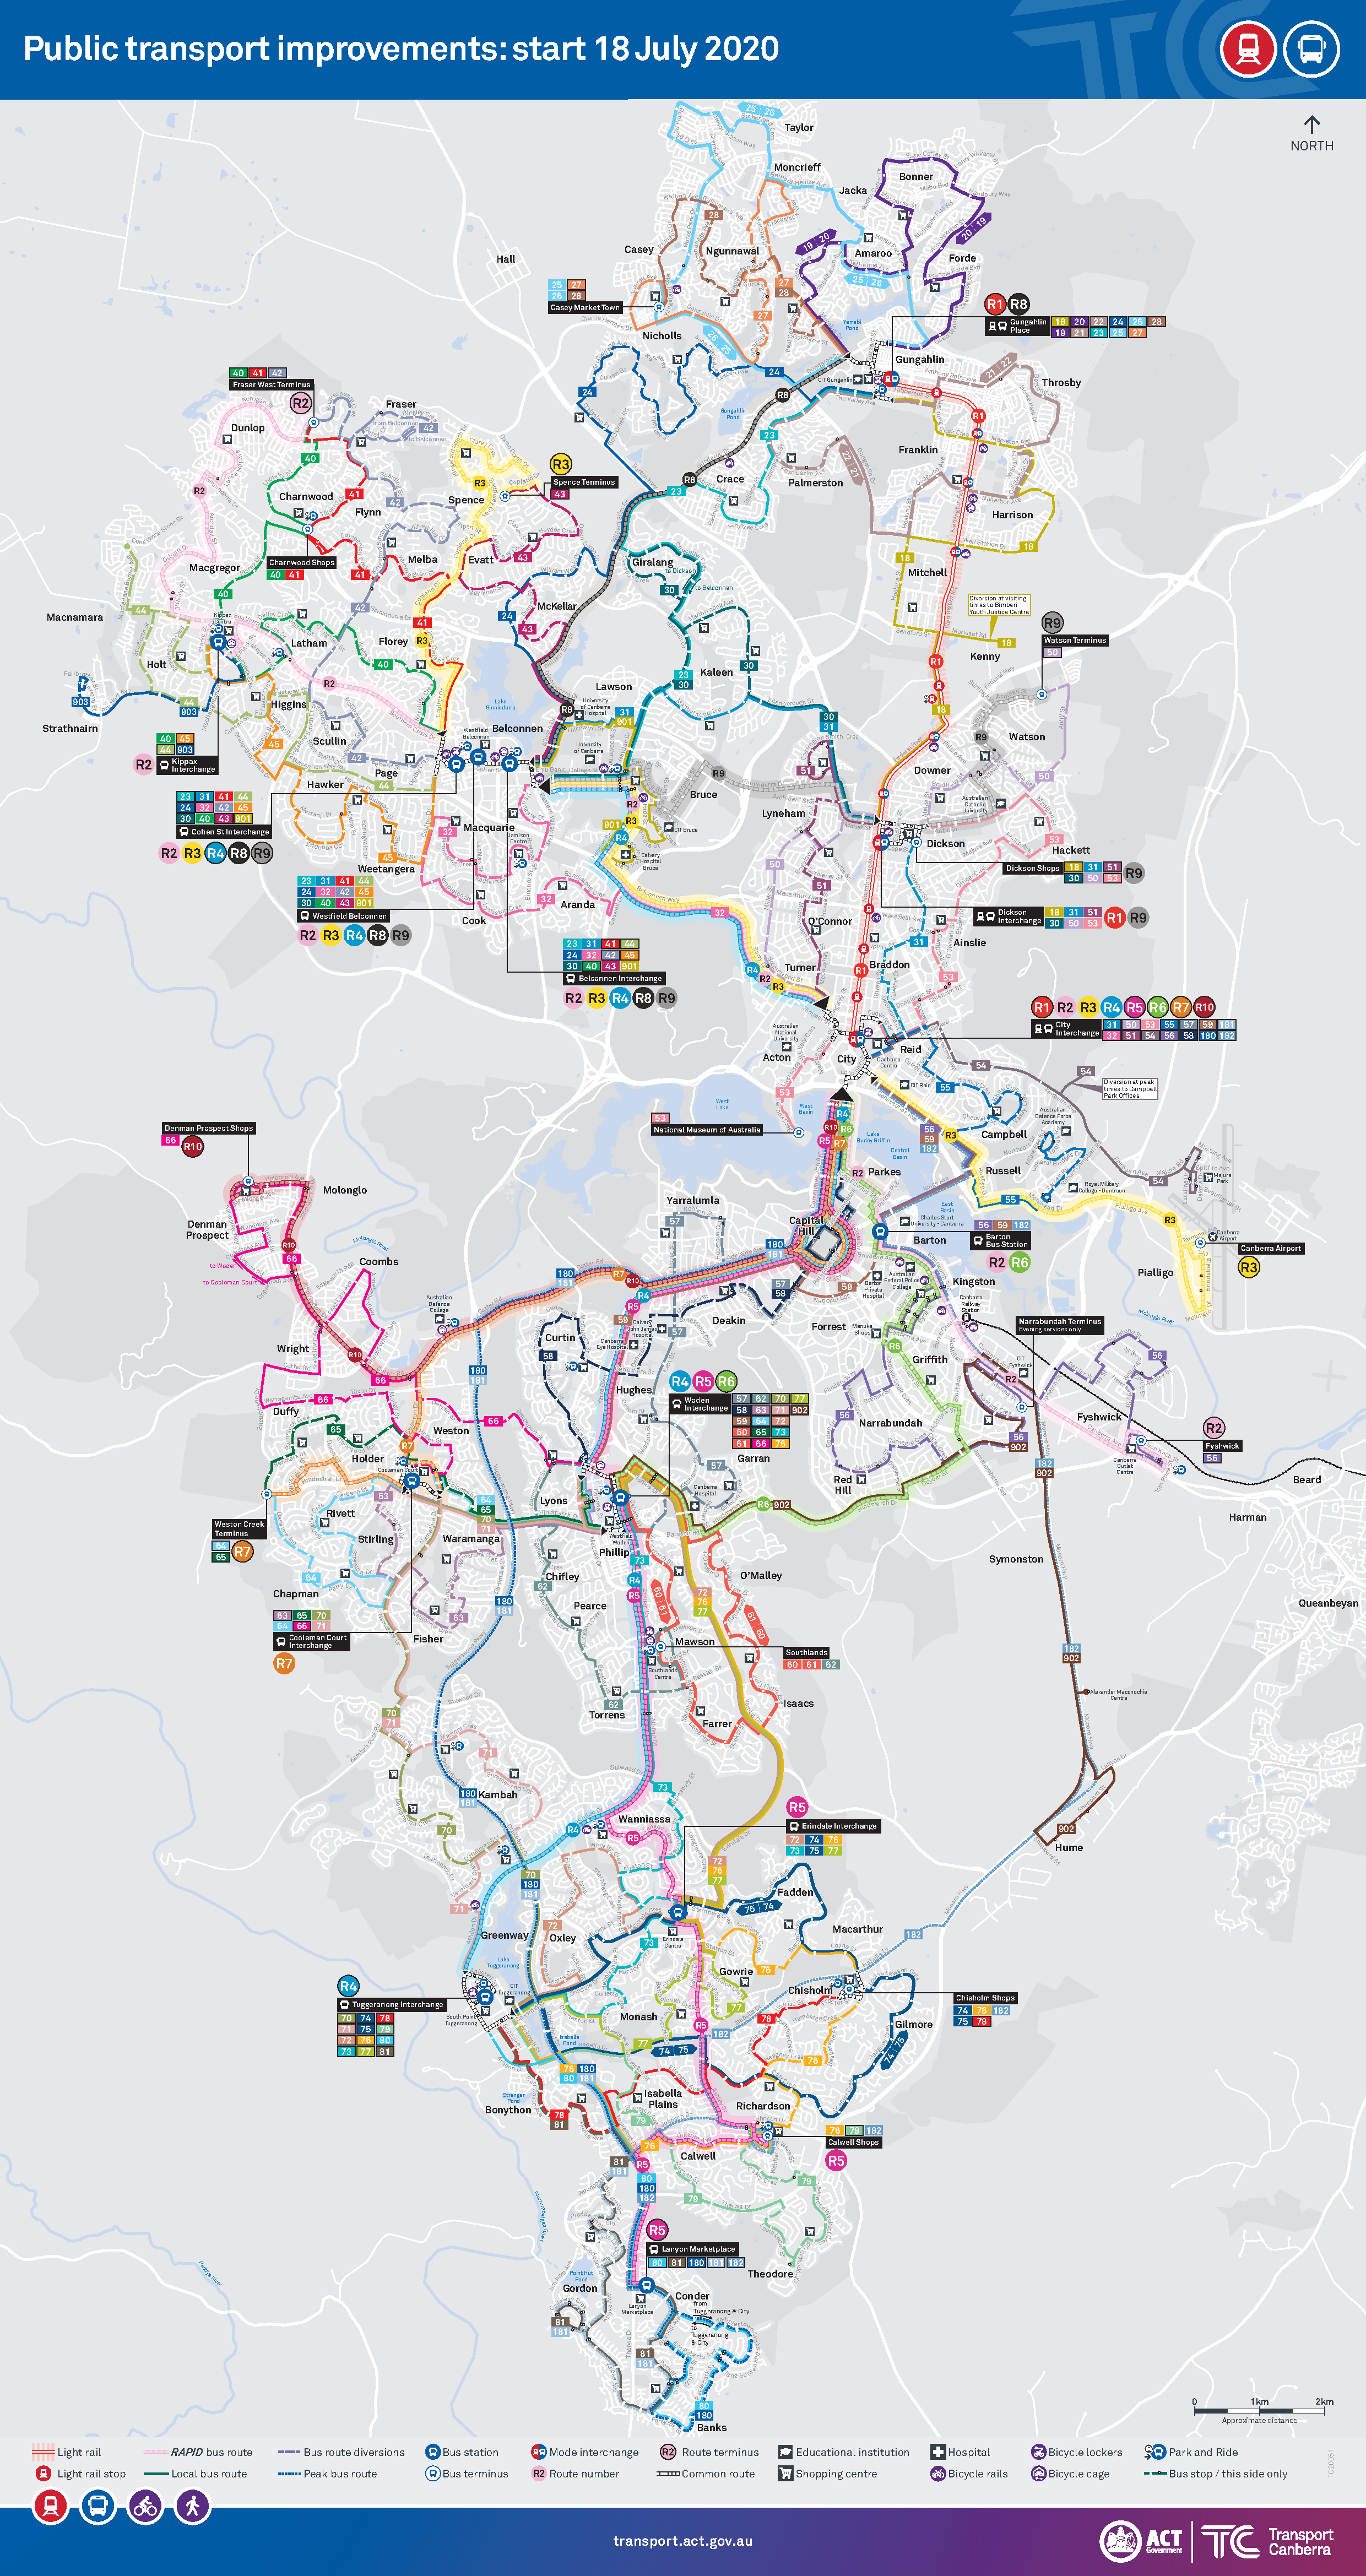
\includegraphics[scale=0.20]{assets/CanberraMap}
		\rule{16cm}{0.4pt} \\
		\vspace{5mm}
		
\includegraphics[scale=0.20]{assets/logoISEP} \\
		\textsc{\large Sarah HEOUAINE - David LAMY-VERDIN - Elia TSO}
		\medbreak
		\textsc{\large 2020 - 2021}
	\end{center}
\end{titlepage}

\renewcommand{\contentsname}{Table of contents}
\tableofcontents
\cleardoublepage

\section{Introduction}

\subsection{City of choice}

	We selected the city of Canberra, capital of Australia, for our project. This city has a total of 2433 stations and 2759 links.
	
\subsection{Goals of the project}

	This project had for first goal to create a graph representing the transport map of Canberra out of mere data. After this graph has been created, we could use it to reach other goals described in the below list:
	
\begin{itemize}
\item[-] Search algorithms \\
Implementation of the Bread-First Search Algorithm \\
Implementation of the Dijkstra Algorithm
\medbreak
\item[-] Applications of those algorithms \\
Searching for shortest paths \\
Splitting the map into clusters
\end{itemize}

	Through this project, optimization also had to be done as searching for shortest paths and splitting into clusters a graph as large as Canberra Transport Map was particularly demanding on resources and took a considerable amount of time.
	
\subsection{Collection of data : GTFS files}
	
	To build our graph, we used data retrieved from \href{https://www.transport.act.gov.au/contact-us/information-for-developers}{Australia Government official website}. This data come as multiple \textit{.txt} files. After studying them, it has been figured out that only \textit{stops.txt} and \textit{stop\_times.txt} were actually useful.
	
\begin{center}
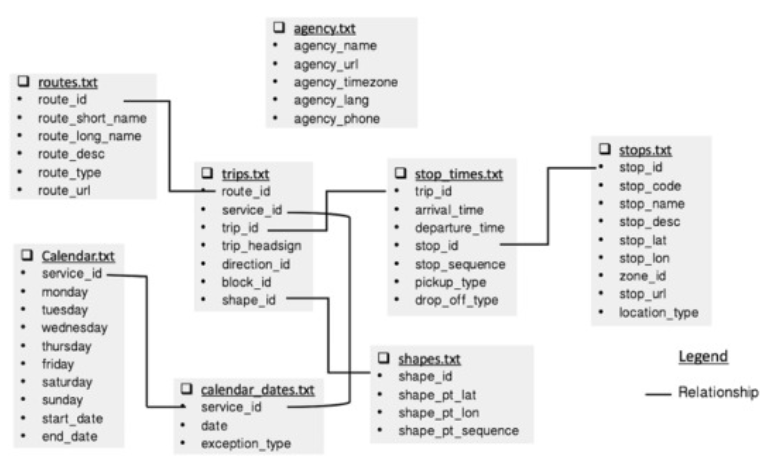
\includegraphics[scale=1]{assets/data}
\end{center}

	Using only those, we could create the stations which are represented in our graph as nodes and we could also link each of them and thus creating our edges.
	
\newpage
	
	The \textit{stops.txt} file provide us with \textit{stop\_id},  \textit{stop\_lat}, \textit{stop\_lon} which are all the information we needed to create our nodes while the \textit{stop\_times.txt} give us \textit{trip\_id} which allow us to create our edges. A trip informs about which stations are linked together and in which order as it defines a bus or subway line such as the R3 line of Canberra for example:
\begin{center}
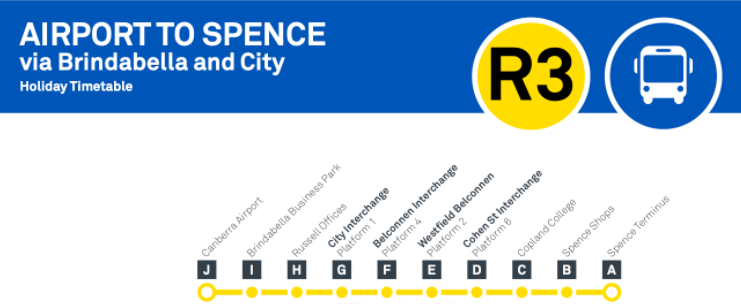
\includegraphics[scale=1]{assets/R3}
\end{center}

\section{Creation of the graph}

\subsection{Graph}

\mintinline{java}{Graph.java} is the class used for building graphs.
The class contains the three following attributes:

\begin{itemize}
\item[-]\mintinline{java}{private Map<Integer, List<DirectedEdge>> map = new TreeMap<Integer,List<DirectedEdge>>()} which are the adjacency lists of every node of our graphs. Each \mintinline{java}{Key} of the \mintinline{java}{Map} designates a node of our graph and the corresponding \mintinline{java}{Value} of the \mintinline{java}{Map} is its adjacency list.
\item[-]\mintinline{java}{private boolean weighted} indicates if the graph is weighted or not.
\item[-]\mintinline{java}{private boolean directed} indicates if the graph is directed or not.
\end{itemize}

	Besides these attributes, \mintinline{java}{Graph.java} also has several methods whose most important ones are the following:

\begin{itemize}
\item[-]\mint{java}{private void addNodesFromTxt(File stopsFile)}
\item[-]\mint{java}{private void addEdgesFromTxt(File stopTimesFile)}
\item[-]\mint{java}{private void addWeightsFromTxt(File stopsFile)}
\end{itemize}

All of these methods are used to parse \textit{stops.txt} and \textit{stop\_times.txt}, retrieve the data and create the content of our graph which are nodes and edges.



\begin{comment}
\begin{minted}[breaklines]{java}
public static void dijkstra(Graph G, int startingNode) {
	List<Integer> toVisitNodes = new ArrayList<Integer>();
	toVisitNodes.add(startingNode);
	previous.put(startingNode, startingNode);
	distance.put(startingNode, 0.0);
		
	if (verifyNonNegative(G)) {
		for (Integer key : G.getMap().keySet()) {
			if (key != startingNode) {
				marked.put(key, false);
				distance.put(key, Double.POSITIVE_INFINITY); //999999999 is supposed to be infinity
			}	
		}
			
		boolean end = false;
		
		while (!end) {
			end = false;
			double minimalDistance = Double.POSITIVE_INFINITY;
			int currentNode = startingNode;
			// With the for loop below, we choose our node with the minimal distance as our next node
			for (int i = 0 ; i < toVisitNodes.size() ; i ++) {
				if (distance.get(toVisitNodes.get(i)) < minimalDistance) {
					minimalDistance = distance.get(toVisitNodes.get(i));
					currentNode = toVisitNodes.get(i);
				}
				// We select our next node and remove it from toVisitNodes
				toVisitNodes.remove((Integer)currentNode);
			}
			// We set our node as marked after it is selected and removed from toVisitNodes
			marked.put(currentNode, true);
				
			for (DirectedEdge edge : G.getMap().get(currentNode)) {
					// We update the distance of the neighbors nodes
					// We check the distance, if they are shorter, we change it, if not, we do not
				if (distance.get(edge.to()) > distance.get(edge.from()) + edge.weight()) {
					distance.put(edge.to(), distance.get(edge.from()) + edge.weight());
					previous.put(edge.to(), edge.from());						
						
					}
					// We take care not to select again a marked node
				if (!marked.get(edge.to())) {
					toVisitNodes.add(edge.to());
				}
			}
			
				// If there is not any node left to visit, we stop the loop
			if (toVisitNodes.isEmpty()) end = true;
		}
	} else {
		System.out.println("Dijkstra algorithm cannot be used as there is a negative weight in the graph!");
	}
}
\end{minted}
\end{comment}
\end{document}
